\documentclass{beamer}
\usepackage{amsmath}
\usepackage{moreverb}
\usepackage{amssymb}
\usepackage{graphicx}
\usepackage{mathtools}
\usepackage{tikz}
\usepackage{pgfplots}
\usetikzlibrary{arrows,shapes, positioning}
\DeclarePairedDelimiter\floor{\lfloor}{\rfloor}
\let\biconditional\leftrightarrow
\newenvironment{customlegend}[1][]{%
    \begingroup
    % inits/clears the lists (which might be populated from previous
    % axes):
    \csname pgfplots@init@cleared@structures\endcsname
    \pgfplotsset{#1}%
}{%
    % draws the legend:
    \csname pgfplots@createlegend\endcsname
    \endgroup
}%

% makes \addlegendimage available (typically only available within an
% axis environment):
\def\addlegendimage{\csname pgfplots@addlegendimage\endcsname}

\pgfkeys{/pgfplots/number in legend/.style={%
        /pgfplots/legend image code/.code={%
            \node at (0.295,-0.0225){#1};
        },%
    },
}
\begin{document}
    \begin{frame}
    \frametitle{Webservices Architecture}
        The architecture of the webservices distributed system is as follows
                \begin{equation}
            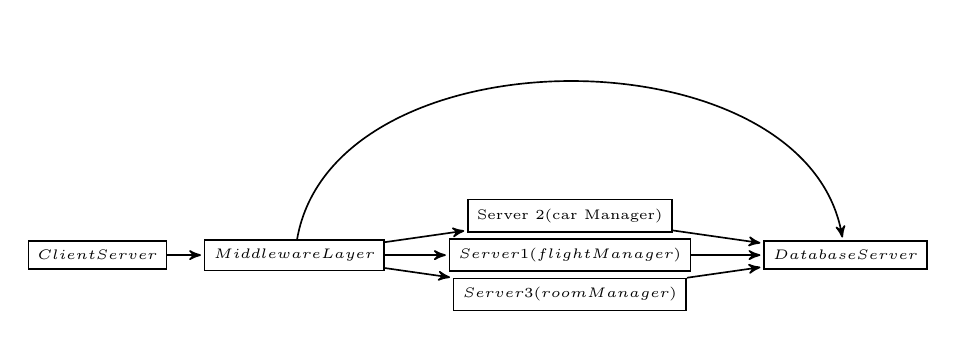
\begin{tikzpicture}[->,>=stealth',shorten >=1pt,auto,node distance=0.5cm,semithick]
            \node[draw] (rect)                  (A)                 {\tiny{$Client Server$}};
            \node[draw] (rect)                  (B) [right of=A,xshift=2cm] {\tiny{$Middleware Layer$}};
            \node[draw] (rect)        (C) [right of=B,xshift=3cm] {\tiny{$Server 1(flight Manager)$}};
            \node[draw] (rect) (D)[above of=C] {\tiny{Server 2(car Manager)}}; 
            \node[draw] (rect)    (E)[below of=C] {\tiny{$Server 3(room Manager)$}};
            \node[draw] (rect)    (F)[right of = C, xshift=3cm]{\tiny{$Database Server$}}; 
            

            \path 
            (A) edge              node{}  (B)
            (B) edge              node {} (C)
                edge              node {} (D)
                edge              node {} (E)
                edge[out=80,in=100]  node {} (F)
            (C) edge              node {}(F)
            (D) edge              node {}(F)
            (E) edge              node {} (F); 
            \end{tikzpicture}
            \end{equation}
    \end{frame}
    \begin{frame}
    \frametitle{Sockets Implementration:}

    The overaching architecture of the websockets code is identical to the structure shown in (1). As such the description will be focused on the
    implementations of webservices on top of websockets. \\
    We begin by creating an executor service and oppening a websocket. The server then listens on the socket of all incomming connections, once a connection is opened it is accpted and
    packaged into a request context which contains a RequestManager and the socket connection. The request manager implements runnable and is passed to the executor service which assigns the connection a thread and invokes Request Manager's run. The executor service guarantees that connections are run asynchronously and act as a threadpool. \\
    \end{frame}
    \begin{frame}
    \frametitle{Sockets Implementation:}
    The RequestManager's run fetches the socket from the request context, upon receiving an input stream we use Java builtin serialization to pass our own request and response objects,
    this allows us to gracefully handle exceptions in a network transparent manner. The Resquest Handler of the recipient then uses Java's build in reflection toolset to identify which method should be invoked providing us with a method of remote method invocation through sockets. As per the webservices code database access is handled through DBCP connection pools. 
    \end{frame}
    \begin{frame}
    \frametitle{Sockets Implementation}
    The resource managers thus have the following set of relations. 
    \begin{equation}
    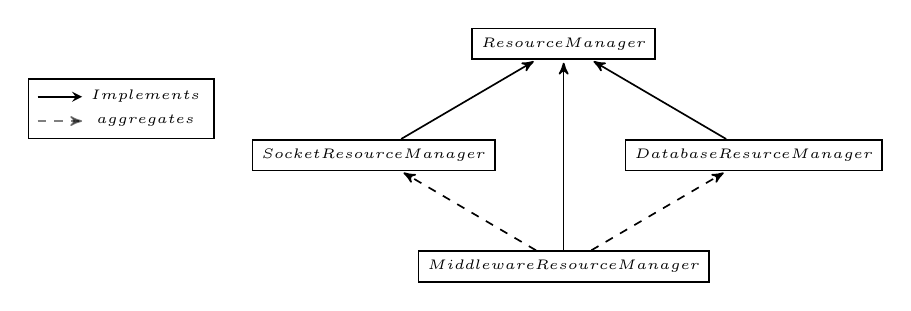
\begin{tikzpicture}[->,>=stealth',shorten >=1pt,auto,node distance=2cm,semithick]
        \node[draw] (rect) (A)[xshift=3cm] {\tiny{$SocketResourceManager$}};
        \node[draw] (rect) (B) [above right of=A,xshift=1cm] {\tiny{$ResourceManager$}};
        \node[draw] (rect) (C) [below right of=B, xshift=1cm]{\tiny{$DatabaseResurceManager$}};
        \node[draw] (rect) (D) [below right of=A, xshift=1cm]{\tiny{$MiddlewareResourceManager$}}; 
        \path
        (A) edge node{} (B)
        (B)
        (C) edge node{} (B)
        (D) edge node{} (B)
            edge[dashed] node{} (C)
            edge[dashed] node{} (A);
        \begin{customlegend}[
            legend entries={ % <= in the following there are the entries
            \tiny{$Implements$},
            \tiny{$aggregates$}
            }] % <= to define position and font legend
            % the following are the "images" and numbers in the legend
            \addlegendimage{-stealth,black,opacity=1}
            \addlegendimage{black,dashed,opacity=0.5}
            \end{customlegend} 
     \end{tikzpicture}
     \end{equation}
    \end{frame}
    \begin{frame}
    \frametitle{Shared Design}
        Shared design between the webservices and Sockets implementations is restricted to the POSTGRESQL database
        which is identical in both cases and has the following schema. 
        \begin{equation}
             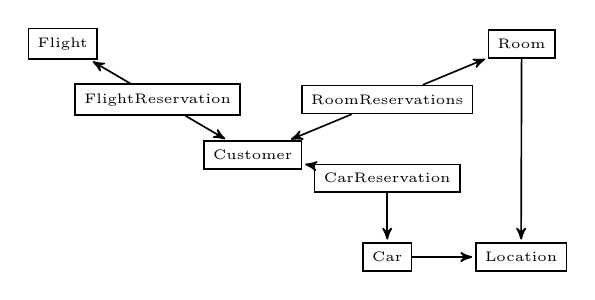
\begin{tikzpicture}[->,>=stealth',shorten >=1pt,auto,node distance=1cm,semithick]
             \node[draw] (rect)     (A) {\tiny{Flight}};
             \node[draw] (rect)     (B) [below right of=A,xshift=0.5cm] {\tiny{FlightReservation}};
             \node[draw] (rect)     (C) [below right of=B,xshift=0.5cm] {\tiny{Customer}};
             \node[draw] (rect)     (D) [above right of=C,xshift=1cm] {\tiny{RoomReservations}};
             \node[draw] (rect)     (E) [below of=D] {\tiny{CarReservation}};
             \node[draw] (rect)     (F) [below of=E] {\tiny{Car}};
             \node[draw] (rect)     (G) [right of=F,xshift=0.70cm] {\tiny{Location}}; 
             \node[draw] (rect)     (H) [above right of=D, xshift=1cm]{\tiny{Room}}; 
             \path
             (A)
             (B) edge node{} (A)
                edge  node{}  (C)
             (C)
             (D) edge node{} (C)
                 edge node{} (H)
             (E) edge node{} (C)
                 edge node{} (F)
             (F) edge node{} (G)
             (G)
             (H) edge node{} (G); 
             \end{tikzpicture}
             \end{equation}
    \end{frame}
\end{document}